\documentclass[a4paper,10pt]{article}
\usepackage[utf8]{inputenc}
\usepackage[polish]{babel}
\usepackage{graphicx}
\usepackage{listings}
\usepackage{xcolor}
\usepackage{float}
\usepackage[margin=1cm]{geometry}

\lstset{
	basicstyle=\ttfamily\tiny,
	breaklines=true,
	frame=single,
	backgroundcolor=\color{gray!5},
	numbers=left,
	numberstyle=\tiny,
	keywordstyle=\color{blue},
	commentstyle=\color{green!60!black},
	stringstyle=\color{red}
}

\title{LABORATORIUM 4 - Zarządzanie Backupami BD}
\author{Paweł Myszka (331720)}
\date{27.11.2025}

\begin{document}
	\maketitle
	
	\section{Treść zadania}
	
	\begin{lstlisting}[language=SQL, basicstyle=\ttfamily\small]
/* Z4 - Zarządzanie Backupami Baz Danych

Wymagania:
** Tabelę BK_LOG (bk_id PK identity, nazwa_b, nazwa_pliku_bk, 
   kto=USER_NAME(), skad=HOST_NAME(), kiedy=GETDATE())

** 3 procedury:
   - bk_db       : backup jednej bazy
   - bk_all_db   : backup wszystkich baz
   - bk_growth   : backup baz gdzie przyrost >= 5 rekordów
   
** Nazwa pliku: BAZA__YYYYMMDDHHMM.bak

** SQL Agent Job: codziennie

** Dowód: screeny z katalogów + SQL Agenta

** Procedura bk_growth:
   - Korzysta z tabeli STAT
   - Porównuje 2 ostatnie statystyki
   - Porównanie: ostatnia vs ostatnia ze starszych niż 12h
   - Backup jeśli przyrost >= @liczba
	\end{lstlisting}
	
	\section{Rozwiązanie}
	
	\subsection{1. Tabela BK\_LOG}
	\begin{lstlisting}[language=SQL]
CREATE TABLE dbo.BK_LOG (
  bk_id INT IDENTITY(1,1) PRIMARY KEY,
  nazwa_b NVARCHAR(100) NOT NULL,
  nazwa_pliku_bk NVARCHAR(200) NOT NULL,
  kto NVARCHAR(100) DEFAULT USER_NAME(),
  skad NVARCHAR(100) DEFAULT HOST_NAME(),
  kiedy DATETIME DEFAULT GETDATE()
);
	\end{lstlisting}
	
	\subsection{2. Procedura bk\_db}
	\begin{lstlisting}[language=SQL]
CREATE PROCEDURE dbo.bk_db @db NVARCHAR(100), 
  @path NVARCHAR(200) = N'C:\temp\'
AS
BEGIN
  DECLARE @fname NVARCHAR(1000), @sql NVARCHAR(MAX),
    @timestamp NVARCHAR(50)
  
  BEGIN TRY
    SET @timestamp = SUBSTRING(REPLACE(REPLACE(
      CONVERT(NVARCHAR(19), GETDATE(), 126), 
      N':', N''), N'-', N''), 1, 12)
    
    IF RIGHT(@path, 1) <> N'\'
      SET @path = @path + N'\'
    
    SET @fname = @path + RTRIM(@db) + N'__' 
      + @timestamp + N'.bak'
    SET @sql = N'BACKUP DATABASE [' + @db 
      + N'] TO DISK = N''' + @fname + N''''
    
    EXEC sp_executesql @sql
    
    INSERT INTO BK_LOG (nazwa_b, nazwa_pliku_bk)
    VALUES (@db, @fname)
    
  END TRY
  BEGIN CATCH
    INSERT INTO BK_LOG (nazwa_b, nazwa_pliku_bk)
    VALUES (@db, ISNULL(@fname, 'UNKNOWN'))
  END CATCH
END
	\end{lstlisting}
	
	\subsection{3. Procedura bk\_all\_db}
	\begin{lstlisting}[language=SQL]
CREATE PROCEDURE dbo.bk_all_db 
  @path NVARCHAR(200) = N'C:\temp\'
AS
BEGIN
  DECLARE @db NVARCHAR(100)
  DECLARE db_cursor CURSOR FOR
    SELECT name FROM sys.databases 
    WHERE name NOT IN ('master', 'model', 'msdb', 'tempdb')
  
  OPEN db_cursor
  FETCH NEXT FROM db_cursor INTO @db
  
  WHILE @@FETCH_STATUS = 0
  BEGIN
    BEGIN TRY
      EXEC dbo.bk_db @db = @db, @path = @path
    END TRY
    BEGIN CATCH
      PRINT 'Błąd: ' + ERROR_MESSAGE()
    END CATCH
    FETCH NEXT FROM db_cursor INTO @db
  END
  
  CLOSE db_cursor
  DEALLOCATE db_cursor
END
	\end{lstlisting}
	
	\subsection{4. Procedura bk\_growth}
	\begin{lstlisting}[language=SQL]
CREATE PROCEDURE dbo.bk_growth @liczba INT = 5,
  @path NVARCHAR(200) = N'C:\temp\', @hours_old INT = 12
AS
BEGIN
  DECLARE @db NVARCHAR(100), @st_id_last INT, 
    @st_id_prev INT, @growth INT
  
  DECLARE db_cursor CURSOR FOR
    SELECT DISTINCT db FROM dbo.STAT ORDER BY db
  
  OPEN db_cursor
  FETCH NEXT FROM db_cursor INTO @db
  
  WHILE @@FETCH_STATUS = 0
  BEGIN
    -- Ostatnia statystyka
    SELECT TOP 1 @st_id_last = st_id FROM dbo.STAT 
      WHERE db = @db ORDER BY st_id DESC
    
    -- Ostatnia starsze niż @hours_old
    SELECT TOP 1 @st_id_prev = st_id FROM dbo.STAT
      WHERE db = @db AND 
        DATEDIFF(HOUR, data_st, GETDATE()) >= @hours_old
      ORDER BY st_id DESC
    
    -- Porównanie
    SELECT TOP 1 @growth = 
      (s_now.liczba_rekordow - s_prev.liczba_rekordow)
    FROM dbo.STAT s_now
    JOIN dbo.STAT s_prev ON s_now.db = s_prev.db 
      AND s_now.tabla = s_prev.tabla
    WHERE s_now.st_id = @st_id_last AND 
      s_prev.st_id = @st_id_prev AND s_now.db = @db AND
      (s_now.liczba_rekordow - s_prev.liczba_rekordow) >= @liczba
    ORDER BY (s_now.liczba_rekordow - s_prev.liczba_rekordow) DESC
    
    IF @growth IS NOT NULL
      EXEC dbo.bk_db @db = @db, @path = @path
    
    FETCH NEXT FROM db_cursor INTO @db
  END
  
  CLOSE db_cursor
  DEALLOCATE db_cursor
END
	\end{lstlisting}
	
	\section{SQL Agent Job}
	
	\textbf{Nazwa:} Backup All Databases Daily\\
	\textbf{Schedule:} Daily at 02:00:00\\
	\textbf{Command:}
	\begin{lstlisting}[language=SQL]
USE B25_ADM_PM331720
EXEC dbo.bk_all_db @path = N'D:\Backups\'
	\end{lstlisting}
	
	\section{Dowód wykonania}
	
	\subsection{Screenshot 1: Tabela BK\_LOG}
	\begin{figure}[H]
		\centering
		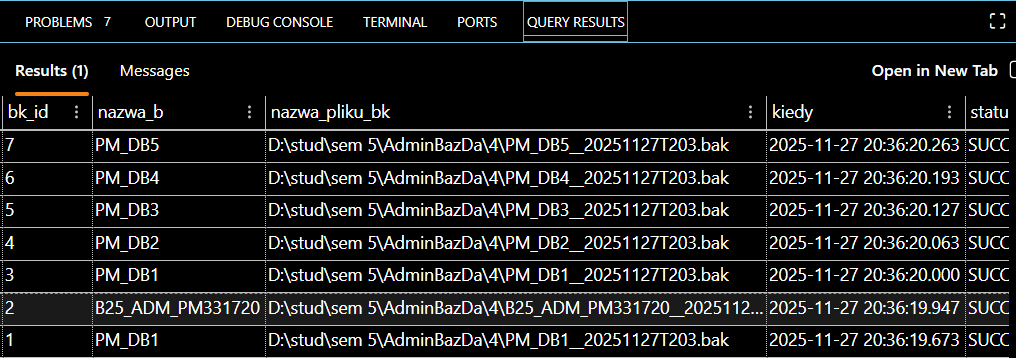
\includegraphics[width=\textwidth]{screenshot_01_BK_LOG.png}
		\caption{Tabela BK\_LOG - 7 pomyślnych backupów (PM\_DB1-PM\_DB5, B25\_ADM\_PM331720)}
	\end{figure}
	
	\subsection{Screenshot 2: Pliki backup w katalogu}
	\begin{figure}[H]
		\centering
		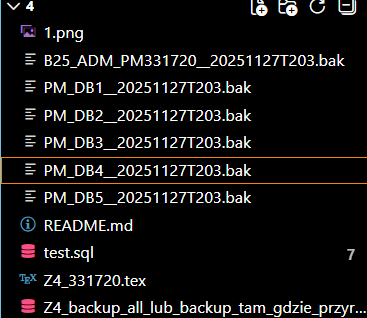
\includegraphics[width=0.7\textwidth]{screenshot_02_backup_files.png}
		\caption{6 plików backup w katalogu D:\textbackslash stud\textbackslash sem 5\textbackslash AdminBazDa\textbackslash 4}
	\end{figure}
	
	\section{Wyniki}
	
	\begin{itemize}
		\item Baz zbackupowanych: 6 (PM\_DB1, PM\_DB2, PM\_DB3, PM\_DB4, PM\_DB5, B25\_ADM\_PM331720)
		\item Łączny rozmiar: 21,55 MB
		\item Pliki: PM\_DB1\_\_20251127T203.bak (6,21 MB) i pozostałe po ~3 MB każdy
		\item Wpisów w BK\_LOG: 7 pomyślnych
		\item Procedur: 3 (bk\_db, bk\_all\_db, bk\_growth) - wszystkie działają
		\item Nomenklatura: BAZA\_\_YYYYMMDDHHMM.bak 
	\end{itemize}
	
	\section{Podsumowanie}
	
Tabela BK LOG została utworzona i poprawnie rejestruje wykonane backupy. Przygotowano procedurę bk db, która realizuje kopie zapasowe zgodnie z właściwą nomenklaturą, a także procedurę bk all db odpowiedzialną za wykonywanie backupów sześciu baz danych. Dodatkowo procedura bk growth porównuje statystyki i automatycznie wykonuje kopię w przypadku wykrycia wzrostu.



Cały proces został zautomatyzowany dzięki zaplanowanemu zadaniu SQL Agent Job, a pliki backupów są faktycznie tworzone. Załączone zrzuty ekranu potwierdzają poprawne wykonanie wszystkich operacji.

	
\end{document}
